\documentclass{article}
\usepackage[utf8]{inputenc}
\usepackage{scrextend}
\usepackage{amsfonts}
\usepackage{amssymb}
\usepackage{tikz}
\usepackage{siunitx}
\usepackage[T2A]{fontenc}
\usepackage[english]{babel}
\def\frak#1{\cal #1}
\usepackage{amssymb,amsmath}
\usepackage{graphicx}
\usepackage{alltt}
\usepackage{enumitem}
\usepackage{chessboard}
\usepackage{skak}
\setcounter{secnumdepth}{1}

\title{Решения на задачите от контролно 1 по Логическо програмиране}
\date{17 ноември 2018}

\begin{document}
\maketitle

\section{Определелимост}
Нека ${\cal L}=\langle p\rangle$ е език с за предикатно смятане с формално равенство, имащ само един нелогически символ - двуместният предикатен символ p.\\ ${\cal{A}}=\langle ChessBoard; p^{\cal{A}}\rangle$ е структура за ${\cal L}$, където под \textit{ChessBoard} разбираме множеството от всички наредени полета от стандартната шахматна дъска (от \texttt{a1} до \texttt{h8}).  

\subsection{Вариант 1}
За всеки два елемента a и b на \textit{ChessBoard}:
\begin{center}
$p^A(a, b) \iff$ от полето a с кон може за един ход да се отиде в полето b.
\end{center}

\begin{enumerate}[label=(\roman*)]
\item Определете множеството от всички ъглови полета.
\item Определете множеството от всички периферни полета.
\item Докажете, че  в тази структура множеството \texttt{\{a2\}} е неопределимо.
\end{enumerate}

\subsection{Вариант 2}
За всеки три елемента a, b и c на \textit{ChessBoard}:
\begin{center}
$p^A(a, b, c) \iff$ от полето a с кон може за един ход да се отиде в полето b или в полето c.
\end{center}

\begin{enumerate}[label=(\roman*)]
\item Определете множеството от всички ъглови полета.
\item Определете множеството от всички периферни полета.
\item Докажете, че  в тази структура множеството \texttt{\{a1\}} е неопределимо.
\end{enumerate}

\begin{center}
\begin{frame}
\newgame
\setchessboard{showmover=false}
\chessboard[setfen=8/8/8/3N4/8/8/8/8 w - - 0 0,
            pgfstyle=border,markfields={c3,e3,b4,f4,b6,f6,c7,e7},
            markfield={d5}] 
\end{frame}
\end{center}

\subsection{Примерно решение:}
За вариант 2 лесно можем да минем към вариант 1:\\
$\varphi_{neighbour}(a, b) \rightleftharpoons p(a, b, b)\\
\varphi_{has\_two\_neighbours}(a) \rightleftharpoons \exists b \exists c (\neg (b \doteq c) \& p(a, b) \& p(a, c) \& \\ \indent \forall d(p(a,d) \Longrightarrow (d \doteq b \lor d \doteq c)))\\
\varphi_{has\_three\_neighbours}(a) \rightleftharpoons \exists b \exists c \exists d(\neg (b \doteq c) \& \neg (c \doteq d) \& \neg(b \doteq d) \& \\ \indent  p(a, b) \& p(a, c) \& p(a, d) \&\forall e(p(a,e) \Longrightarrow (e \doteq b \lor e \doteq c \lor e \doteq d)))\\
\varphi_{has\_four\_neighbours}(a) \rightleftharpoons \exists b \exists c \exists d \exists e (\neg (b \doteq c) \& \neg (c \doteq d) \& \neg(b \doteq d) \&  \\ \indent \neg(e \doteq b) \& \neg(e \doteq c) \& \neg(e\doteq d)\&  p(a, b) \& p(a, c) \& p(a, d) \& p(a, e)\& \\ \indent \forall f(p(a,f) \Longrightarrow (f \doteq b \lor f \doteq c \lor f \doteq d \lor f \doteq e)))\\
\varphi_{edge\_fields}(a) \rightleftharpoons \varphi_{has\_two\_neighbours}(a)\\
\varphi_{peripheral\_fields}(a) \rightleftharpoons (\varphi_{has\_two\_neighbours}(a) \lor \varphi_{has\_three\_neighbours}(a) \lor \\ \indent (\varphi_{has\_four\_neighbours}(a) \& \neg \exists b \exists c (\neg (b \doteq c) \& p(a,b) \& p(a,c) \& \\ \indent \varphi_{has\_four\_neighbours}(b) \& \varphi_{has\_four\_neighbours}(c)))\\$

Можем да разгледаме \textit{ChessBoard} като множество от наредени двойки $\{<letter, number> |\ letter \in \{a,b,c,d,e,f,g,h\} \&\ number \in \{1,2,3,4,5,6,7,8\}\}$.
Автоморфизмът може да бъде ротация на \ang{180}. \\
Нека $k$ е автоморфизъм от \textit{ChessBoard} в \textit{ChessBoard} като: 

\[   
k(<letter, number>) = 
     \begin{cases}
       \text{<h, 9-number>, } &\quad\text{if letter == a}\\
       \text{<g, 9-number>, } &\quad\text{if letter == b}\\
       \text{<f, 9-number>, } &\quad\text{if letter == c}\\
       \text{<e, 9-number>, } &\quad\text{if letter == d}\\
       \text{<d, 9-number>, } &\quad\text{if letter == e}\\
       \text{<c, 9-number>, } &\quad\text{if letter == f}\\
       \text{<b, 9-number>, } &\quad\text{if letter == g}\\
       \text{<a, 9-number>, } &\quad\text{if letter == h}\\
     \end{cases}
\]
Имаме, че $k = k^{-1}$ и не променяме дали едно поле е достижимо от друго с един ход на коня т.е. е в сила, че за всеки a и b от \textit{ChessBoard} \\ $p^A(a, b) \iff p^A(k(a), k(b))$. Взимаме огледалния образ на дъската. Така, ако $a1\in$\texttt{\{a1\}}, то $k(a1)=h8 \notin $\texttt{\{a1\}} и следователно \texttt{\{a1\}} не е определимо. Аналогично за вариант 1.



\newpage
\section{Изпълнимост}
Да се докаже, че е изпълнимо множеството, съставено от следните формули:

\subsection{Вариант 1}

$\exists x \forall y \exists z ( p(x,y) \Longrightarrow (p(x,x) \lor (p(y,z) \lor \neg p(x,z))))\\
\forall x \forall y (p(x,y) \Longrightarrow q(x, y))\\
\exists x (\exists y q(x,y) \& \exists y \neg q(x,y))$

\subsection{Вариант 2}

$\exists x \forall y  ( \neg p(x,y) \lor p(x,x) \lor \exists z(p(y,z) \lor \neg p(x,z)))\\
\neg \exists y \exists x (p(y,x) \& \neg q(y, x))\\
\exists y \exists z \exists x (q(x,y) \& \neg q(x,z))$

\subsection{Примерно решение:}
\begin{center}
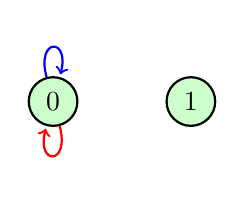
\begin{tikzpicture}[->,,auto,node distance=1.75cm,
                thick,main node/.style={draw, circle, fill=green!20}]

  \node[main node] (0) {0};
  \node[main node] (1) [right of=0] {1};

  \path
    (0) edge [red, loop below] node {} (0)
    (0) edge [blue, loop above] node {} (0);
\end{tikzpicture} \\
$ S = ( \{0, 1 \}, \textcolor{red}{p^S}, \textcolor{blue}{q^S})$ \\
$ \textcolor{red}{p^S} = \{ (0,0) \} $ \\
$ \textcolor{blue}{q^S} = \{ (0,0) \} $
\end{center}


\end{document}
